\documentclass{article}

\usepackage{graphicx}
\usepackage{tikz}
\usepackage{tikzsymbols}
\usetikzlibrary{calc,patterns,shapes.geometric}
\pagestyle{empty}
\usepackage[margin=0pt]{geometry}
\geometry{papersize={14in,12in}}

\def\centerarc[#1](#2)(#3:#4:#5){\draw[#1] ($(#2)+({#5*cos(#3)},{#5*sin(#3)})$) arc (#3:#4:#5);}

\begin{document}
	\begin{figure}
		\centering
		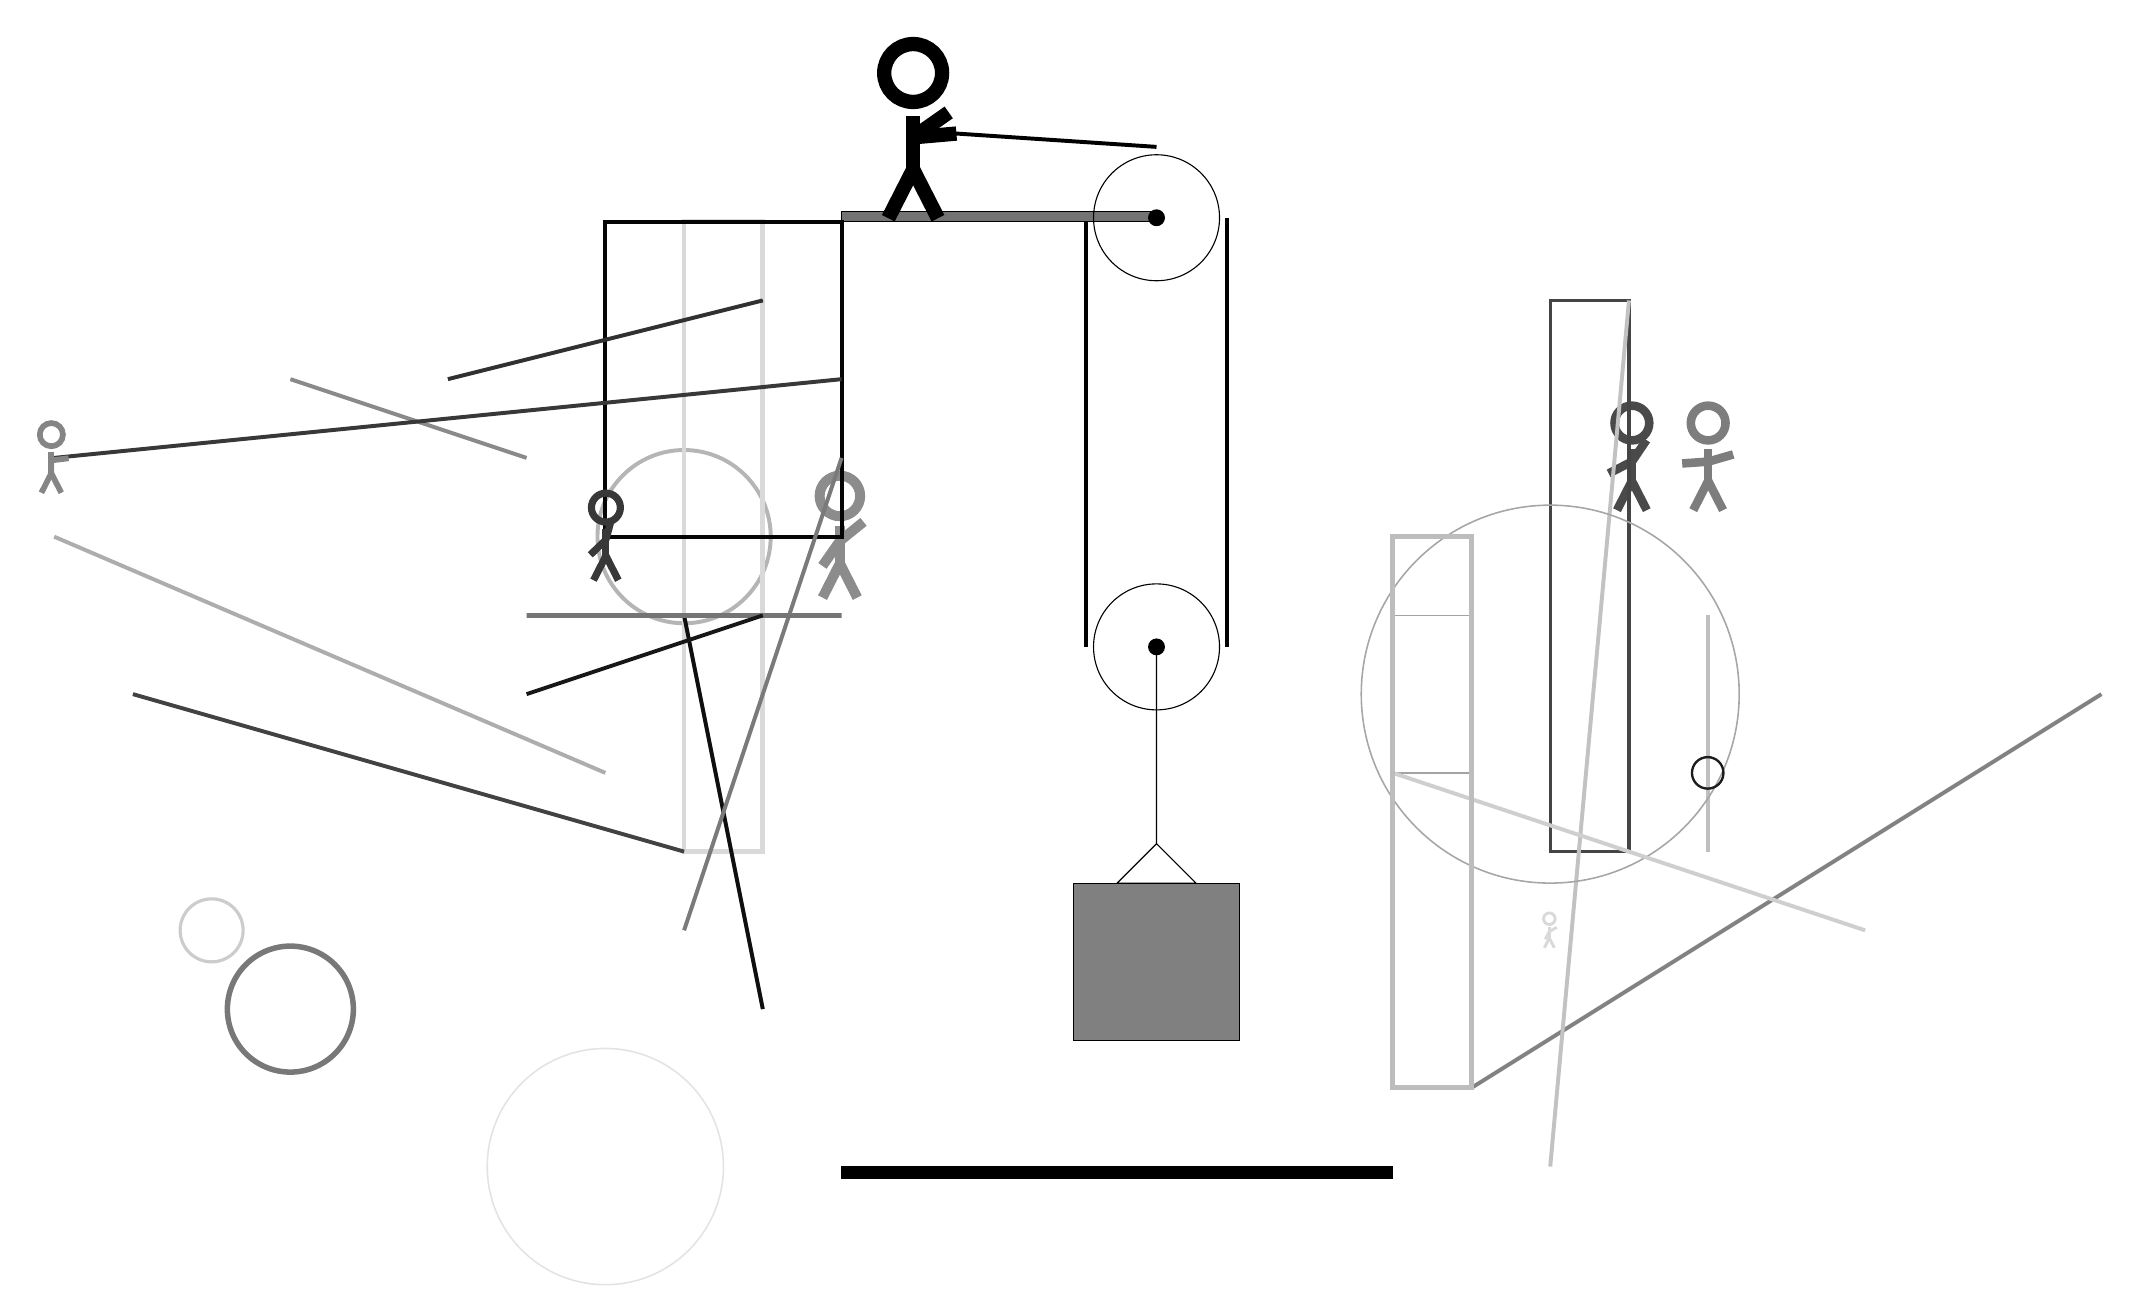
\begin{tikzpicture}
			%%%%% START %%%%%
			
			\draw[fill=black!55] (-2, 9) rectangle (2, 9.125);
			
			\node[line width=0.2mm, color=black!45] at (-2, 5) {\Strichmaxerl[7][55][39]};
			
			\draw [line width=0.5mm, color=black!29](-4, 5) circle (1.1);
			\draw [line width=0.4mm, color=black!20](-10, 0) circle (0.4);
			\node[line width=0.4mm, color=black!71] at (8, 6) {\Strichmaxerl[6][27][56]};
			\draw[line width=0.5mm, color=black!32](-5, 2) -- (-12, 5);
			
			\draw[line width=0.6mm, color=black!15] (-3, 9) rectangle (-4, 1);
			\draw[line width=0.5mm, color=black!49](6, -2) -- (14, 3);
			\draw[line width=0.4mm, color=black!73] (7, 8) rectangle (8, 1);
			\draw[line width=0.5mm, color=black!46](-6, 6) -- (-9, 7);
			\draw[line width=0.5mm, color=black!98] (-2, 9) rectangle (-5, 5);
			\node[line width=0.3mm, color=black!51] at (9, 6) {\Strichmaxerl[6][4][16]};
			\draw[line width=0.5mm, color=black!25](9, 1) -- (9, 4);
			\draw[line width=0.5mm, color=black!78](-2, 7) -- (-12, 6);
			
			\draw[line width=0.5mm, color=black!94](-3, -1) -- (-4, 4);
			\draw [line width=0.7mm, color=black!53](-9, -1) circle (0.8);
			\draw[line width=0.5mm, color=black!52](-4, 0) -- (-2, 6);
			
			\draw[line width=0.5mm, color=black!24](7, -3) -- (8, 8);
			\draw [line width=0.6mm, color=black!42](-4, 1) circle (0.0);
			\draw[line width=0.5mm, color=black!74](-4, 1) -- (-11, 3);
			
			\draw[line width=0.6mm, color=black!54] (-2, 4) rectangle (-6, 4);
			\node[line width=0.7mm, color=black!78] at (-5, 5) {\Strichmaxerl[5][44][75]};
			
			\draw [line width=0.2mm, color=black!35](7, 3) circle (2.4);
			\draw[line width=0.2mm, color=black!36] (5, 2) rectangle (6, 4);
			\draw [line width=0.2mm, color=black!11](-5, -3) circle (1.5);
			\node[line width=0.3mm, color=black!48] at (-12, 6) {\Strichmaxerl[4][89][7]};
			
			\draw[line width=0.5mm, color=black!19](5, 2) -- (11, 0);
			\node[line width=0.6mm, color=black!15] at (7, 0) {\Strichmaxerl[2][62][30]};
			\draw[line width=0.5mm, color=black!81](-7, 7) -- (-3, 8);
			
			\draw [line width=0.3mm, color=black!89](9, 2) circle (0.2);
			\draw[line width=0.6mm, color=black!26] (5, -2) rectangle (6, 5);
			\draw[line width=0.5mm, color=black!91](-3, 4) -- (-6, 3);
			
			
			\draw (2, 3.6) circle (0.8);
			\draw[fill=black] (2, 3.6) circle (0.1);
			
			\draw (2, 9.05) circle (0.8);
			\draw[fill=black] (2, 9.05) circle (0.1);
			
			\draw (2, 3.6) -- (2, 1.1) -- (1.5, 0.6) -- (2.5, 0.6) -- (2, 1.1);
			\draw[fill=black!50] (0.95, 0.6) rectangle (3.05, -1.4);
			
			\draw[line width=0.5mm] (1.1, 9) -- (1.1, 3.6);
			\centerarc[line width=0.5mm](2, 3.6)(180:360:0.9);
			\draw[line width=0.5mm](2.9, 3.6) -- (2.9, 9.05);
			\centerarc[line width=0.5mm](2, 9.05)(0:90:0.9);
			\draw[line width=0.5mm](2, 9.95) -- (-1, 10.15);
			
			\node at (-1, 10.15) {\Strichmaxerl[10][-175][35]};
			
			\draw[fill=black] (-2, -3) rectangle (5, -3.15);
			
			%%%%% END %%%%%
		\end{tikzpicture}
	\end{figure}	
\end{document}